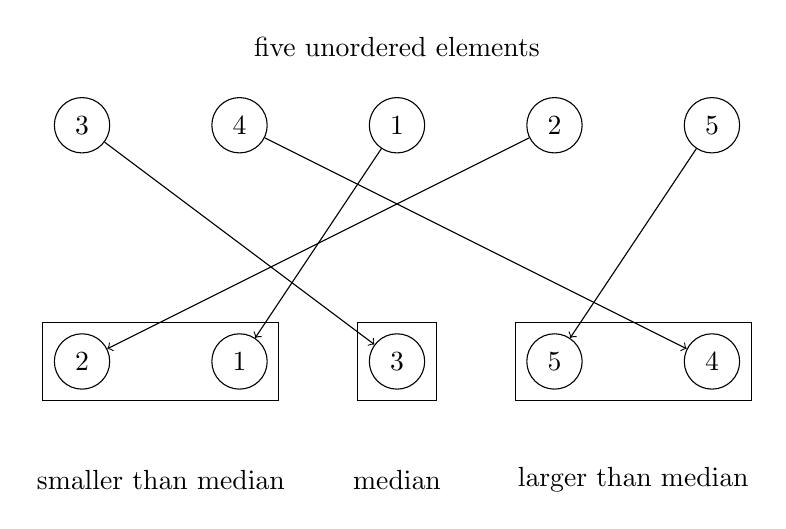
\begin{tikzpicture}

\node [shape=circle, draw=black, minimum size=2em] (v1) at (-3,1.5) {3};
\node [shape=circle, draw=black, minimum size=2em] (v3) at (-1,1.5) {4};
\node [shape=circle, draw=black, minimum size=2em] (v5) at (1,1.5) {1};
\node [shape=circle, draw=black, minimum size=2em] (v7) at (3,1.5) {2};
\node [shape=circle, draw=black, minimum size=2em] (v9) at (5,1.5) {5};
\node [shape=circle, draw=black, minimum size=2em] (v8) at (-3,-1.5) {2};
\node [shape=circle, draw=black, minimum size=2em] (v6) at (-1,-1.5) {1};
\node [shape=circle, draw=black, minimum size=2em] (v2) at (1,-1.5) {3};
\node [shape=circle, draw=black, minimum size=2em] (v10) at (3,-1.5) {5};
\node [shape=circle, draw=black, minimum size=2em] (v4) at (5,-1.5) {4};
\draw [->] (v1) edge (v2);
\draw [->] (v3) edge (v4);
\draw [->] (v5) edge (v6);
\draw [->] (v7) edge (v8);
\draw [->] (v9) edge (v10);
\node at (1,-3) {median};
\node at (-2,-3) {smaller than median};
\node at (4,-3) {larger than median};
\draw [->] (-3.5,-1) rectangle (-0.5,-2);
\draw [->] (2.5,-1) rectangle (5.5,-2);
\draw [->] (0.5,-1) rectangle (1.5,-2);
\node at (1,2.5) {five unordered elements};
\end{tikzpicture}